\documentclass[12pt,a4paper]{article}
\renewcommand{\thesection}{\Roman{section}}
\renewcommand{\thesubsection}{\thesection.\Roman{subsection}}
\usepackage{xeCJK}
\usepackage{caption}
\usepackage{amssymb}
\usepackage{amsmath}
\usepackage{geometry}
\usepackage{subfigure}
\usepackage{fancyhdr}
\usepackage[export]{adjustbox}
\usepackage{graphicx}
\graphicspath{{images/}}
\geometry{left=2.5cm,right=1.5cm,top=2cm,bottom=2cm}

\title{Deep Learning and Practice \\Lab7 \\ Report}
\date{May 30, 2019}
\author{呂紹篁, 0751904}
\setCJKmainfont{AR PL UKai CN}
\begin{document}
\captionsetup[figure]{labelfont={bf},labelformat={default},labelsep=period,name={Fig.}}
\thispagestyle{plain}
\cfoot{}
\maketitle

\section{Intoduction} \label{sec:intro}
In this lab, we will use \textbf{temperal difference}, especially TD(0), a method in reinforcement learning 
for learning the \textbf{value of a state}, to build a bot to play 2048.

\section{Experiment Setups} \label{sec:exp_setup}
\subsection{Temperal Difference}
At timestamp t, the environment state is $s_t$, the value of this state is defined as the expected \textbf{return $G_t$} of the process. 
With \textbf{Bellman equation}, it can be decomposed into two parts: \\ 
\begin{equation}
\begin{split}
v(s_t) & = \mathbb{E}[G_t|S=s_t] \\
       & = \mathbb{E}[R_{t+1}+\gamma R_{t+2}+\gamma^2 R_{t+3}+...|S=s_t] \\
       & = \mathbb{E}[R_{t+1}+\gamma (R_{t+2}+\gamma R_{t+3}+...)|S=s_t] \\
       & = \mathbb{E}[R_{t+1}+\gamma G_{t+1}|S=s_t] \\
       & = \mathbb{E}[R_{t+1}+\gamma v(s_{t+1})|S=s_t]
\end{split}
\end{equation}
TD(0) is a method that update $V(s_t)$ toward estimated return $R_{t+1}+\gamma V(S_{t+1})$, which is called as TD target. \\
The equation for updating $V(s_t)$ can be written as:
\begin{equation}
V(s_t) \leftarrow V(s_t) + \alpha (R_{t+1}+V(s_{t+1})-V(s_t))
\end{equation}
where $\alpha$ is \textbf{learning rate}, and the last term is called 
\textbf{TD error}.
\subsection{After-state and Before-state}
In 2048, after we do an action (that is, up, right, down or left), it not only changes the board, but also 
generates a random 2-tile or 4-tile in unoccupied grid, with probability 0.9 and 0.1
respectively. We call the board after we do some action and before the random tile
is generated as \textbf{after-state} (s' in Fig.\ref{fig:after_before}) and call the board after random tile is 
generated as \textbf{before-state} (s'' in Fig.\ref{fig:after_before}).

\begin{figure}[hbt]
\centering
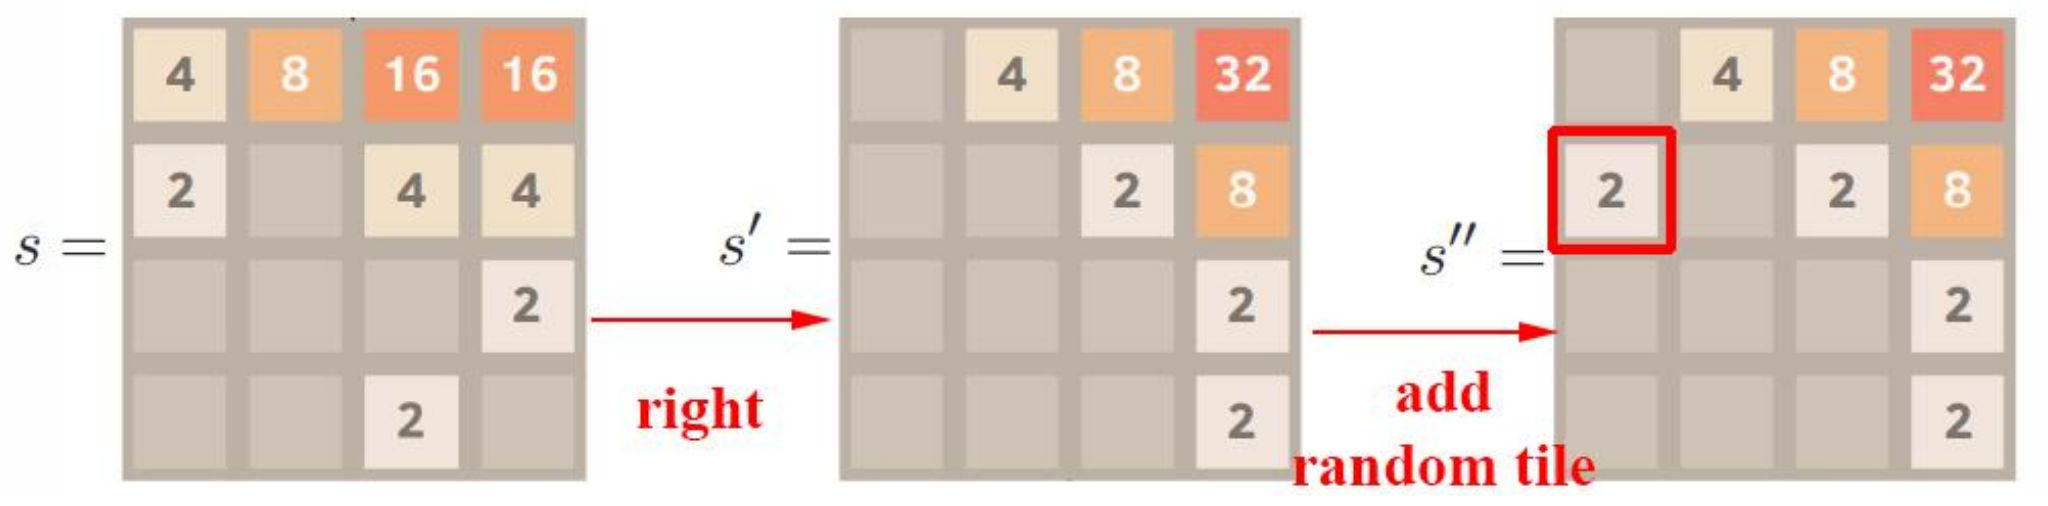
\includegraphics[scale=0.2]{before_after.png}
\caption{Illustration of After-state and Before-state}
\label{fig:after_before}
\end{figure}

\subsection{N-tuple Network}
Consider that every grid will only appear 0 or from $2^1$ to $2^{15}$, then there are 
about $16^{16} = 1.8E19$ states in the state space, which is too huge to compute. 
To reduce the state space and extract the feature from the board effectively, we use
N-tuple netowrk as feature extractor. There are 4 6-tuple in this work, the number of features is $4*16^4 = 6.7E7$, which is much smaller than the one above. Notice also that we will also rotate the board 4 times and mirror. The output of the network is simply the summation of each feature weights.

\subsection{Train a Before-state Network}
The best move for before-state network is to maximize the sum of immediate reward and expected value of state value of before-state. To compute this value, we have to enumerate all possible before-state. This can be done by trace 16 grid value in the after-state, supposes there are 10 empty grid, then 20 possibility may occur, half with 2-tile and the other for 4-tile. To update the state value, since we have played an episode from start state to terminal state (all information (s, a, r, s', s'') are stored in vector \textbf{path}), and it is without doubt that the state value of terminal state is 0, we can therefore compute them recursively with reverse order of path using equation $V(s) \leftarrow V(s) + \alpha (r+V(s'')-V(s))$.

\subsection{Train a After-state Network}
The best move for after-state network is more intuitive and somehow like human behavior in first episode (since we will not give each board a \textit{value}), that is, the agent try to maximize the sum of immediate reward and the state value of after-state after such action. This method is much more computation lightly than before-state since it neglects the consideration of random generated tile. To update the value, since what we care about is after-state, we have to choose the best move of s'' to obtain it. The update follows the equation $V(s') \leftarrow V(s') + \alpha (r_{next} + V(s'_{next}) -V(s'))$ where $s'_{next}, r_{next} \leftarrow COMPUTE_AFTER_STATE(s'', a_{next})$.

\subsection{How the Code Work}
The whole code of C++ version is a messy in first glance since classes are all mixture in one cpp file. While it can break into serveral submodules: 1)in \textit{board} we can get the data of each grid, take action on it and obtain the reward, there are also functions to get the isomorphic board (transpose, mirror, flip, rotate), 2) \textit{feature} define the virtual functions and some basic operators for n-tuple, \textit{pattern}, in the other hand, inherit from feature and implement the functions, 3) \textbf{state} is the wrapper for after-state and before-state, this includes (s, a, r, s'), i.e., before state, action type, reward and after-state, it also contents the value for best move (esti, which can be accessed using function value()), assign function apply the operation toward given board (called before) and step into after, 4) \textbf{learning}, the major backbone for TD learning, after the features are added, we can estimate the state value of given board, update the weight, select the best move ($EVALUATE$ in pseudocode) and update the whole episode ($LEARN\_EVALUATE$), 5) in \textbf{main} function, after basic setup, in given total number of playing times, the agent will start to play and collect data until terminated board met, and using this data to update the state value. \\
Actually, the most important classes are state and learning, and we even don't have to revise \textit{state}, we just have to add two exceed functions in \textit{learning}: select best move and update episode for before-state method.

\section{Experimental Results} \label{sec:res}

\begin{figure}[hbt]
\centering
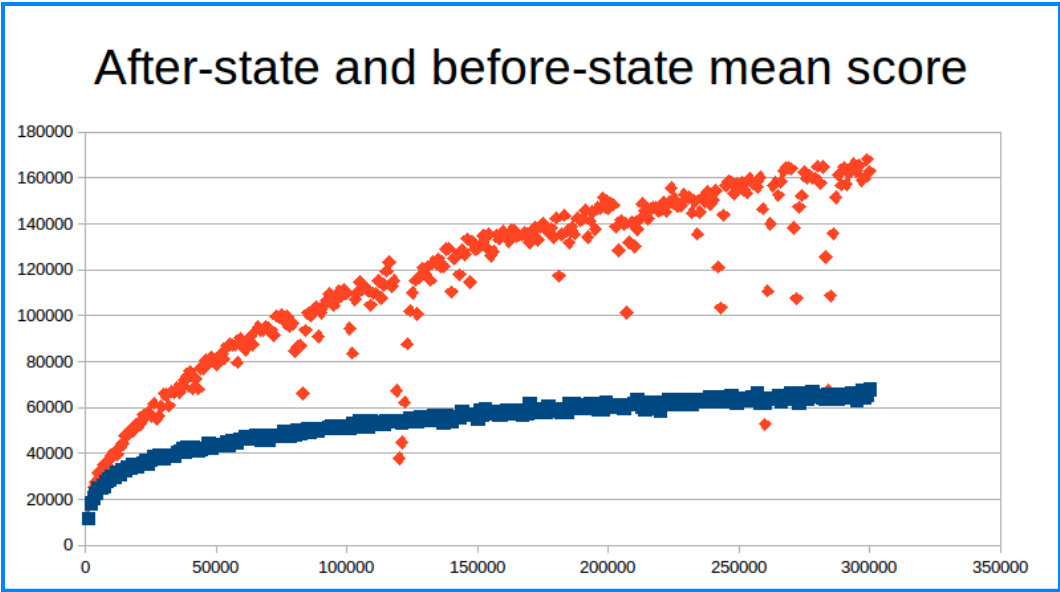
\includegraphics[scale=0.3]{mean_compare.png}
\caption{Comapre of After-state and Before-state Mean Score During 30k Eposides}
\label{fig:compare_mean}
\end{figure}

\begin{figure}[hbt]
\centering
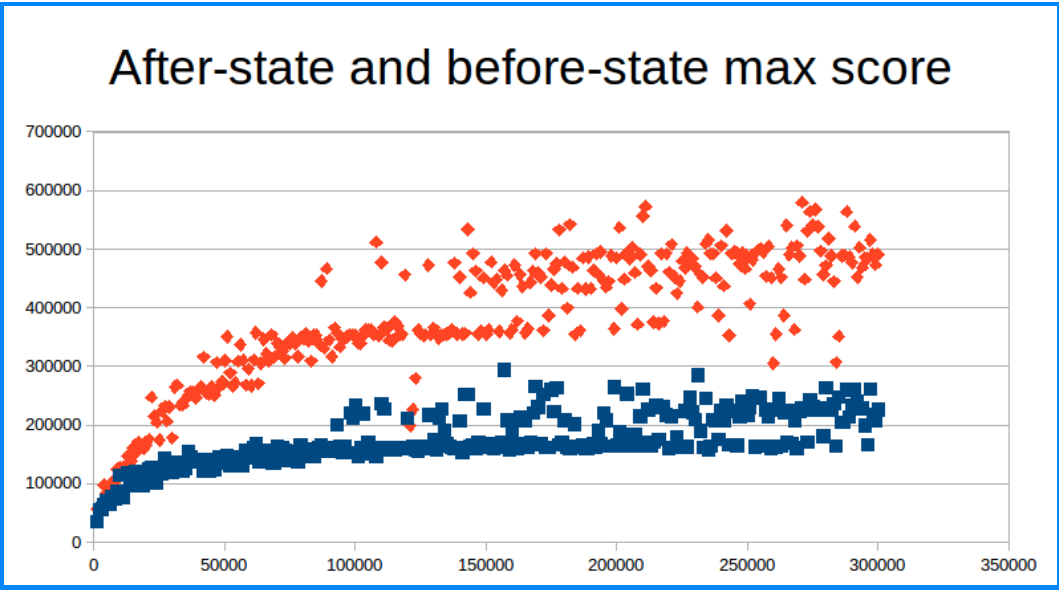
\includegraphics[scale=0.3]{max_compare.png}
\caption{Comapre of After-state and Before-state Maximum Score During 30k Eposides}
\label{fig:compare_max}
\end{figure}

\begin{tabular}{|c|c|}
      \hline
      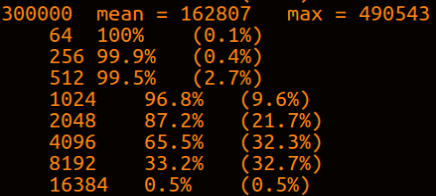
\includegraphics[scale=0.5]{after_state.png} &
      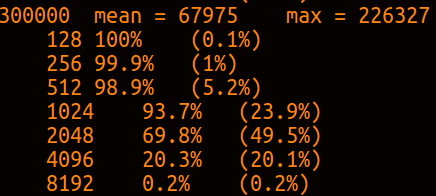
\includegraphics[scale=0.5]{before_state.png} \\
      \small After-state Statistic in Last 1000 Games &  Before-state Statistic in Last 1000 Games \\
      \hline
      
\end{tabular}

\section{Discussion} \label{sec:dis}
\begin{itemize}
\item {Before-state is Much Weaker Than After-state} 
After implement the functions of before-state and start to training, I found that this method is much slower than after-state, after tracing the algorithm, I think that is because in \textit{evaluate}, we have to enumerate all possible situation in given after-state, in the worse case, there are 15*2 = 30 cases, which is more computation heavy. And I also noticed that the mean score is much less than after-state, which the slope of blue curve is less than the orange one in Fig.\ref{fig:compare_mean}. This phenomenon is different from \cite{szubert2014temporal}. I think there maybe some mistakes in my code.
\item {Compare to Q-learning}
In \cite{szubert2014temporal} they also compared two proposed methos with Q-learning framework in Table. II it shown that the result of Q-learning is the worst one among three. While action value is more widely used than state value, in class Prof. Wu also claimed that in Q-learning we don't have to do important sampling, I am not sure why state value estimation is better than action value estimation in this game.
\item {Connect to Website For Better Visualization}
There are several videos in YouTube that playing 2048 in the website with their well-trained agent. Since I want to fool my friends and claim that I can play 2048 very fast and high score, I also cloned the original reposistory and revised the source code. Now I can get the board information from JavaScript and transport a fake keyboard event to cheat the game manager, while the most significant gap is that communicate between C++ and JavaScript. I have found compiler such called Emscripten which can satisfy my need, however I cannot successfully compile my code using this compiler, so I gave up this plan, what a shame!
\end{itemize}

\bibliographystyle{IEEEtran}
\bibliography{report.bib}

\end{document}
